%
% msa.tex
%
% (c) 2019 Prof Dr Andreas Müller, Hochschule Rapperswil
%
\begin{frame}
\frametitle{Multiskalenanalyse}
\begin{center}
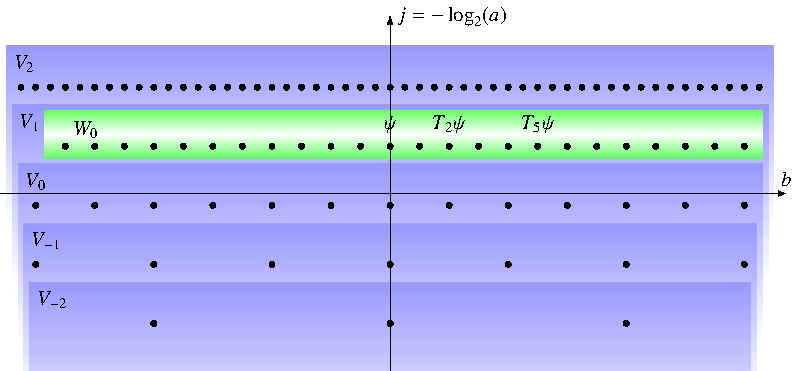
\includegraphics[width=\hsize]{../../buch/chapters/6-msa/images/msa.pdf}
\end{center}
\end{frame}



\begin{frame}
\frametitle{Multiskalenanalyse}
\begin{definition}
Eine {\em Multiskalenanalyse} ist ein Turm von Funktionenräumen
\[
\dots \subset
V_{-2} \subset V_{-1} \subset V_0 \subset V_1 \subset \dots \subset V_j \subset V_{j+1} \subset \cdots 
\]
mit folgenden Eigenschaften:
\begin{enumerate}
\item<2->
Es gibt eine Funktion $\varphi\in V_0$ so, dass die Menge
$\{T_k\varphi\;|\; k\in\mathbb Z\}$ eine orthonormierte Basis von $V_0$ ist:
Vater-Wavelet.
\item<3->
$D_{\frac12}V_j = V_{j+1}$
\item<4->
Der Vektorraum $W_j = \{w\in V_{j+1}\;|\; w\perp v\;\forall v\in V_j\}$
erfüllt $V_{j+1} = V_j \oplus W_j$
\item<5->
Es gibt eine Funktion $\psi\in W_0$ so, dass die Menge
$\{T_k\psi\;|\; k\in\mathbb Z\}$ eine orthonormierte Basis von $W_0$ ist:
Mutter-Wavelet.
\item<6->
$\bigcap_{j\in\mathbb Z} V_j = \{0\}$ und
$\overline{\bigcup_{j\in\mathbb Z}V_j}= L^2(\mathbb R)$
\end{enumerate}
\end{definition}

\end{frame}

%
% Haar-Wavelet als Multiskalen-Analyse
%
\begin{frame}
\frametitle{Haar-Wavelet}

Das Haar-Wavelet erzeugt eine Multiskalen-Analyse:
\uncover<2->{
\begin{columns}[T]
\begin{column}{0.3\hsize}
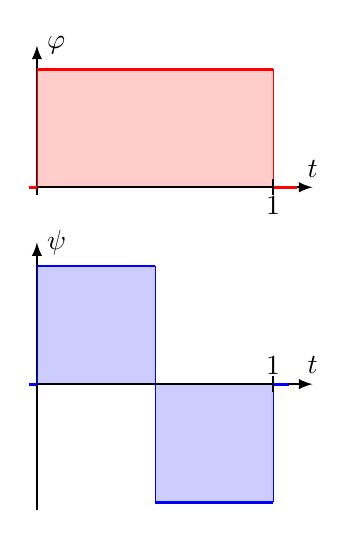
\begin{tikzpicture}[>=latex]
\uncover<3->{%
\fill[color=red!20] (0,0)--(3,0)--(3,1.5)--(0,1.5)--cycle;
\draw[->,line width=0.7pt]
	(-0.1,0)--(3.5,0) coordinate[label={$t$}];
\draw[->,line width=0.7pt]
	(0,-0.1)--(0,1.8) coordinate[label={right:$\varphi$}];
\draw[color=red,line width=1pt] (-0.1,0)--(0,0);
\draw[color=red,line width=0.1pt] (0,0)--(0,1.5);
\draw[color=red,line width=1pt] (0,1.5)--(3,1.5);
\draw[color=red,line width=0.1pt] (3,1.5)--(3,0);
\draw[color=red,line width=1pt] (3,0)--(3.3,0);
\draw[line width=0.7pt] (3,-0.1)--(3,0.1);
\node at (3,0) [below] {$1$};
}

\uncover<5->{%
\begin{scope}[yshift=-2.5cm]
\fill[color=blue!20] (0,0)--(3,0)--(3,-1.5)--(1.5,-1.5)--(1.5,1.5)--(0,1.5)--cycle;
\draw[->,line width=0.7pt]
	(-0.1,0)--(3.5,0) coordinate[label={$t$}];
\draw[->,line width=0.7pt]
	(0,-1.6)--(0,1.8) coordinate[label={right:$\psi$}];
\draw[color=blue,line width=1pt] (-0.1,0)--(0,0);
\draw[color=blue,line width=0.1pt] (0,0)--(0,1.5);
\draw[color=blue,line width=1pt] (0,1.5)--(1.5,1.5);
\draw[color=blue,line width=0.1pt] (1.5,1.5)--(1.5,-1.5);
\draw[color=blue,line width=1pt] (1.5,-1.5)--(3,-1.5);
\draw[color=blue,line width=0.1pt] (3,-1.5)--(3,0);
\draw[color=blue,line width=1pt] (3,0)--(3.2,0);
\draw[line width=0.7pt] (3,-0.1)--(3,0.1);
\node at (3,0) [above] {$1$};
\end{scope}
}

\end{tikzpicture}
\end{column}
\begin{column}{0.61\hsize}
\begin{itemize}
\item<2->
$V_j$ ist der Raum der auf Intervallen $[k2^{-j},(k+1)2^{-j})$ stückweise
konstanten Funktionen
\item<3->
$\varphi$ ist die charakteristische Funktion von $[0,1)$
\item<4->
$\{T_k\varphi\;|\;k\in\mathbb Z\}$ ist eine orthonormierte Basis von $V_j$
\item<5->
$\psi = \frac1{\sqrt{2}} (D_{\frac12}\varphi - D_{\frac12}T_1\varphi)$%
\uncover<6->{,\quad
$\langle\psi,\varphi\rangle=0$}
\item<7->
Die Menge $\{T_k\psi\;|\; k\in\mathbb Z\}$ ist eine Basis $W_0$.
\item<8->
Die stückweise konstanten Funktionen liegen dicht in $L^2(\mathbb R)$
\uncover<9->{%
$\Rightarrow$ $\overline{\bigcup_{j\in\mathbb Z} V_j}=L^2(\mathbb R)$
}
\item<10->
$\bigcap_{j\in\mathbb Z}V_j$ besteht aus den überall konstanten 
$L^2$-Funktionen\uncover<11->{, d.~h.~$\bigcap_{j\in\mathbb Z}V_j=\{0\}$}
\end{itemize}
\end{column}
\end{columns}
}
\end{frame}
